\lstset{language=SQL}

\section{\mt{Adatbázis}{Database}}
\block{
	\subsection{\mt{Áttekintés}{}}

	\p{\mt{%
		A rendszer Mysql relációs adatbázist használ. Az adatbázis létrehozásához szükséges SQL kód a \code{api/db.sql} fájlban található.
		A táblákban sokszor megtalálható az \code{external\_id} attributum, amely az API által használt azonosítót tárolja.
		Erre azért van szükség, mert a valódi azonosító módosításához a táblák nagy részét le kéne zárni, ami lassítaná a
		lekéréseket. Az adatbázisban több nézet is található a lekérések egyszerűbbé tételére.
		Az alábbi grafikon mutatja a táblák kapcsolatrendszerét:
	}{}}
}

\begin{landscape}
	\begin{figure}
		\centering
		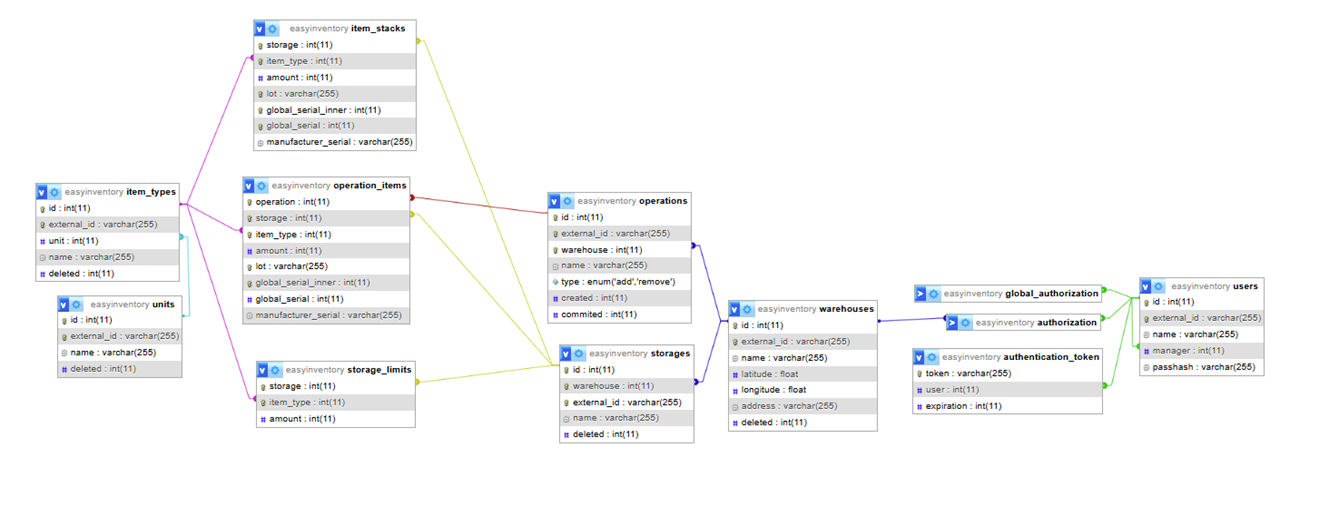
\includegraphics[width=\linewidth]{db.png}
	\end{figure}
\end{landscape}

\block{
	\subsection{\mt{Táblaleírások}{}}
	
	\subsubsection{untis}

	\p{\mt{%
			A \code{units} tábla a mértékegységek tárolásáért felelős.
		}{}
		
		\lstinputlisting{generated/database.units.sql}
	}
}

\block{
	\subsubsection{item\_types}

	\p{\mt{%
			Az \code{item\_types} tábla a különböző cikk típusok tárolásáért felelős.
		}{}
		
		\lstinputlisting{generated/database.item_types.sql}
	}
}

\block{
	\subsubsection{warehouses}

	\p{\mt{%
			A \code{warehouses} tábla a különböző telephelyek tárolásáért felelős.
		}{}
		
		\lstinputlisting{generated/database.warehouses.sql}
	}
}

\block{
	\subsubsection{storages}

	\p{\mt{%
			A \code{storages} tábla a különböző raktárak tárolásáért felelős.
		}{}
		
		\lstinputlisting{generated/database.storages.sql}
	}
}

\block{
	\subsubsection{item\_stacks}

	\p{\mt{%
			Az \code{item\_stacks} tábla az éppen tárolt különböző árucikkek tárolásáért felelős.
		}{}

        \lstinputlisting{generated/database.item_stacks.sql}
	}
}

\block{
	\subsubsection{storage\_limits}

	\p{\mt{%
			A \code{storage\_limits} tábla a raktár limiteket tárolásáért felelős.
		}{}
		
		\lstinputlisting{generated/database.storage_limits.sql}
	}
}

\block{
	\subsubsection{operations}

	\p{\mt{%
			Az \code{operations} tábla a műveletek tárolásáért felelős.
		}{}
		
		\lstinputlisting{generated/database.operations.sql}
	}
}

\block{
	\subsubsection{operation\_items}

	\p{\mt{%
			Az \code{operation\_items} tábla a művelet részek tárolásáért felelős.
		}{}
		
		\lstinputlisting{generated/database.operation_items.sql}
	}
}

\block{
	\subsubsection{users}

	\p{\mt{%
			A \code{users} tábla a felhasználók tárolásáért felelős.
		}{}
		
		\lstinputlisting{generated/database.users.sql}
	}
}

\block{
	\subsubsection{authorization}

	\p{\mt{%
			Az \code{authorization} tábla a helyi engedélyek tárolásáért felelős.
		}{}
		
		\lstinputlisting{generated/database.authorization.sql}
	}
}

\block{
	\subsubsection{global\_authorization}


	\p{\mt{%
			A \code{global\_authorization} tábla a rendszer engedélyek tárolásáért felelős.
		}{}
		
		\lstinputlisting{generated/database.global_authorization.sql}
	}
}

\block{
	\subsubsection{authentication\_token}

	\p{\mt{%
			Az \code{authentication\_token} tábla a bejelentkezési tokenek tárolásáért felelős.
		}{}
		
		\lstinputlisting{generated/database.authentication_token.sql}
	}
}

\block{
	\subsection{\mt{Nézetek}{}}
	
	\subsubsection{users\_view}

	\p{\mt{%
			A \code{users\_view} a felhasználók adatainak lekérését egyszerűsíti.
		}{}
		
		\lstinputlisting{generated/database.users_view.sql}
	}
}

\block{
	\subsubsection{authorization\_view}

	\p{\mt{%
			Az \code{authorization\_view} tábla a helyi és rendszer engedélyek lekérését egyszerűsíti.
		}{}
		
		\lstinputlisting{generated/database.authorization_view.sql}
	}
}

\block{
	\subsubsection{authentication\_token\_view}

	\p{\mt{%
			Az \code{authentication\_token\_view} a bejelentkezési tokenek lekérését egyszerűsíti.
		}{}
		
		\lstinputlisting{generated/database.authentication_token_view.sql}
	}
}

\block{
	\subsubsection{warehouses\_view}

	\p{\mt{%
			A \code{warehouses\_view} tábla a telephelyek lekérését egyszerűsíti.
		}{}
		
		\lstinputlisting{generated/database.warehouses_view.sql}
	}
}

\block{
	\subsubsection{storages\_view}

	\p{\mt{%
			A \code{storages\_view} tábla a raktárak lekérését egyszerűsíti.
		}{}
		
		\lstinputlisting{generated/database.storages_view.sql}
	}
}

\block{
	\subsubsection{item\_types\_view}

	\p{\mt{%
			A \code{item\_types\_view} tábla a cikk típusok lekérését egyszerűsíti.
		}{}
		
		\lstinputlisting{generated/database.item_types_view.sql}
	}
}

\block{
	\subsubsection{units\_view}

	\p{\mt{%
			A \code{units\_view} tábla a mérték egységek lekérését egyszerűsíti.
		}{}
		
		\lstinputlisting{generated/database.units_view.sql}
	}
}

\block{
	\subsubsection{operations\_view}

	\p{\mt{%
			A \code{operations\_view} tábla a műveletek lekérését egyszerűsíti.
		}{}
		
		\lstinputlisting{generated/database.operations_view.sql}
	}
}

\block{
	\subsubsection{operation\_items\_view}

	\p{\mt{%
			A \code{operation\_items\_view} tábla a művelet részek lekérését egyszerűsíti.
		}{}
		
		\lstinputlisting{generated/database.operation_items_view.sql}
	}
}

\block{
	\subsubsection{item\_stacks\_view}

	\p{\mt{%
			A \code{item\_stacks\_view} tábla a tárolt áru lekérését egyszerűsíti.
		}{}
		
		\lstinputlisting{generated/database.item_stacks_view.sql}
	}
}

